\section{Tritium as a Calibration Source} \label{TritiumChapter}


In this chapter, we'll discuss the use of tritium as an internal calibration source in the LUX detector.  The material presented here will focus on the R\&D efforts to produce such a source prior to LUX's Run 3 data taking campaign, as well as the first results from the calibration source during the Run 3 campaign.  Tritium is an ideal calibration source for measuring the detector's electron recoil response, since the the beta decay spans the entire WIMP search energy range.  Note that the source is not a replacement for the mono-energetic $^83m$Kr source which is used to produce signal corrections in Chapter~\ref{StandardCalibrations}, since the wide spectral shape is less suited for tracking position and time dependence of the S1 and S2 signals.  The tritium calibration source was also a critical component in dealing with the non-uniform drift field in LUX's Run 4 data, which will be discussed in Chapter~\ref{Run04Corrections}.

\subsection{Motivation for a Tritium Calibration Source}

In two phase (liquid and gas) xenon detectors ionizing events will produce a scintillation signal (referred to as S1) and ionization. The electrons produced by the ionization process can be drifted to an anode located in the gas phase of the detector. Once the electrons are accelerating toward the anode in the xenon gas they will create a secondary scintillation signal (referred to as S2). Nuclear recoil events have higher ionization density, leading to a higher probability that electron will recombine at the site of the initial recoil event, resulting in a higher S1 yield and lower S2 yield than electron recoil events of the same energy. Therefore, the ratio of the S1 and S2 signals can be used to distinguish electron recoil backgrounds from WIMP-like nuclear recoil events.  This background discrimination technique is referred to as nuclear recoil discrimination.

The number of photons and electrons produced during a nuclear recoil or electron recoil events of a given energy must be well understood to take advantage of nuclear recoil discrimination.  Typically, an external beta emitter such as $^{137}$Cs is used to calibrate the detector's electron recoil response. However, the xenon in LUX has a strong self-shielding characteristic at $\sim$MeV wavelengths. While this is convenient for eliminating background radiation from external sources, it makes calibrating the innermost regions of the detector difficult with external gamma sources.

To overcome this problem, the LUX collaboration makes use of internal calibration sources. An ideal internal calibration source for measuring the electron recoil yields would be a single beta emitter in the energy range of interest (< 15 keV) which can be dissolved into the liquid xenon in the detector. Furthermore, the source must be made of a material with low electronegativity so that it will not diminish the drift length of charge in the detector. Similarly the source cannot attenuate the UV scintillation light produced by events in the detector. To achieve a reliable calibration in all regions of the detector the source should have a long enough lifetime to mix uniformly throughout the entire detector (an hour or more). Finally, there must be a method for removing the source once the calibration has finished. This could simply mean waiting for the source to decay, if its half-life is short, or actively purifying the source out of the detector if its half-life is long

Tritium meets several of these requirements. It is a beta emitter with a Q-value of 18.6 keV, a mean energy of 5.6 keV, and a mode of 3 keV that produces a broad spectrum over the entire energy range of interest. Its 12.3 year half-life means that the source will have plenty of time to mix uniformly throughout the detector. However, this long half life is potentially dangerous, since one can not simply wait for it to decay away. It must be actively removed from the detector when the calibration is completed. To complicate this matter, bare tritium sticks to most surfaces, including materials like teflon, polyethylene, and steel which make up the majority of most xenon detectors. To make tritium removal more feasible we have made use of tritiated methane(CH$_3$T). Methane is highly inert due to its fully saturated carbon-hydrogen bonds. It has a diffusion constant in polyethylene that is 10 times smaller than
hydrogen, and it does not capture electrons that will be drifting through the detector~\cite{TeflonActivationEnergy}. By replacing one of the hydrogen atoms in a methane molecule with tritium we combine the strength of both of these materials, resulting in the ideal internal electron recoil calibration source.

\subsection{Triated Methane Removal} \label{UMDRemoval}

The CH$_4$ removal efficiency of zirconium getters was measured through xenon assaying in 2010~\cite{Dobi:2010ai}. To ensure the CH$_3$T removal efficiency of zirconium getters was similar, we built two separate systems to inject tritiated methane into a gaseous xenon and a liquid xenon environment. Both of these systems used zirconium getters to remove CH$_3$T.  In this section, we describe the resulting measurements and calculations that ensured the successful injection of CH$_3$T into LUX in 2013.

\subsubsection{Gas Phase Experiments}

The gaseous xenon system consists of three sections. The first section, the xenon space, contains a hot zirconium getter to remove CH$_3$T from the system, two xenon storage bottles, and a proportional tube to detect activity within the xenon space.  The two storage bottles are used to move xenon through the system via cryopumping.  The second section is a small transfer system which is used to inject consistent amounts of CH$_3$T into the xenon space with each injection. The final section consists of a CH$_3$T storage bottle and a SAES MC1-905F methane purifier to remove unwanted non-methane contaminates prior to entering the xenon space.  

%Insert gas system diagram here
\begin{figure}
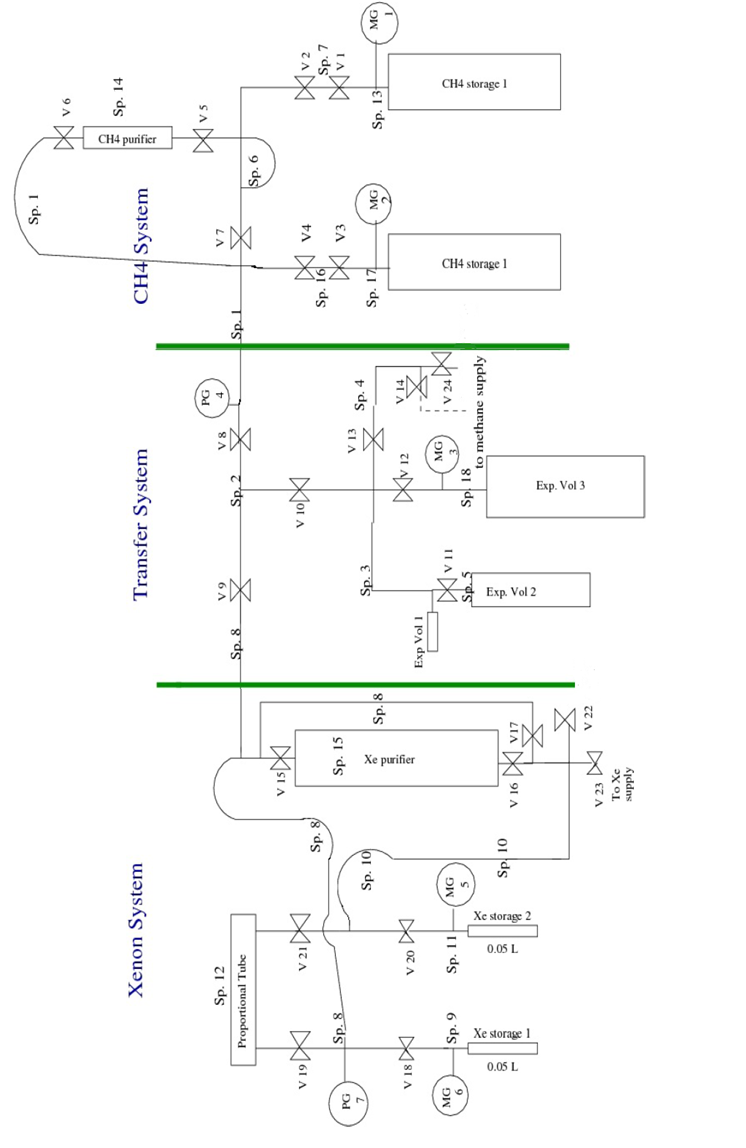
\includegraphics[scale=.55]{GasSystem.png} 
\captionof{figure}{Diagram of the gaseous xenon system at UMD.  The three sections of the system are distinguished by green lines.  Circles labeled PG and MG are pressure gauges, and the hourglass shaped symbols represent hand valves.}
\label{UMDGasSystem}
\end{figure}

The primary goals of this experiment were to determine the purification efficiency of the zirconium getter and to study residual contamination.  As shown in Figures~\ref{UMDGasFlowRate} and~\ref{UMDGasRestTime}, we found that the flow rate through the getter and the amount of time between injections had the largest impact of purification efficiency.  High  flow rates through the purifier can cool the zirconium inside, while inadequate rest time between subsequent purifications can lead to build up of methane on the surface of the zirconium pellets. Both of these situations lead to a modest decrease in purifier efficiency. The first black data point in Figure~\ref{UMDGasFlowRate} is our worst purification efficiency, (96\% $\pm$ 1\%) corresponding to our highest flow rate. (8 SLPM compared to the typical 0.3 SLPM) While we were unable to control the  flow rate as much as we desired, we are at least able to conclude that exceeding the maximum flow rate suggested for the purifier does have a measurable effect on the purification efficiency. We also found that allowing ample rest time between subsequent purifications significantly increases purification efficiency. Our best purifications were the first data points in each cluster in Figure~\ref{UMDGasRestTime}. We were able to obtain efficiencies of 99.99\% when the purifier was resting for three weeks or longer, and obtained efficiencies ranging from 99.00\% to 99.90\% when the purifier was used on a daily basis.  Because of the constant recirculation in LUX, any purification efficiency above 90\% is acceptable.

After dozens of sequential injections, we observed a modest increase in the background activity observed by the proportional tube.  The source of the residual activity was likely contaminates from the CH$_3$T source bottle, such as tritiated water.  To remove these contaminates, a methane purifier was added to the flow path.  After including the methane purifier, the background rate of the proportional tube remained constant.

\begin{figure}
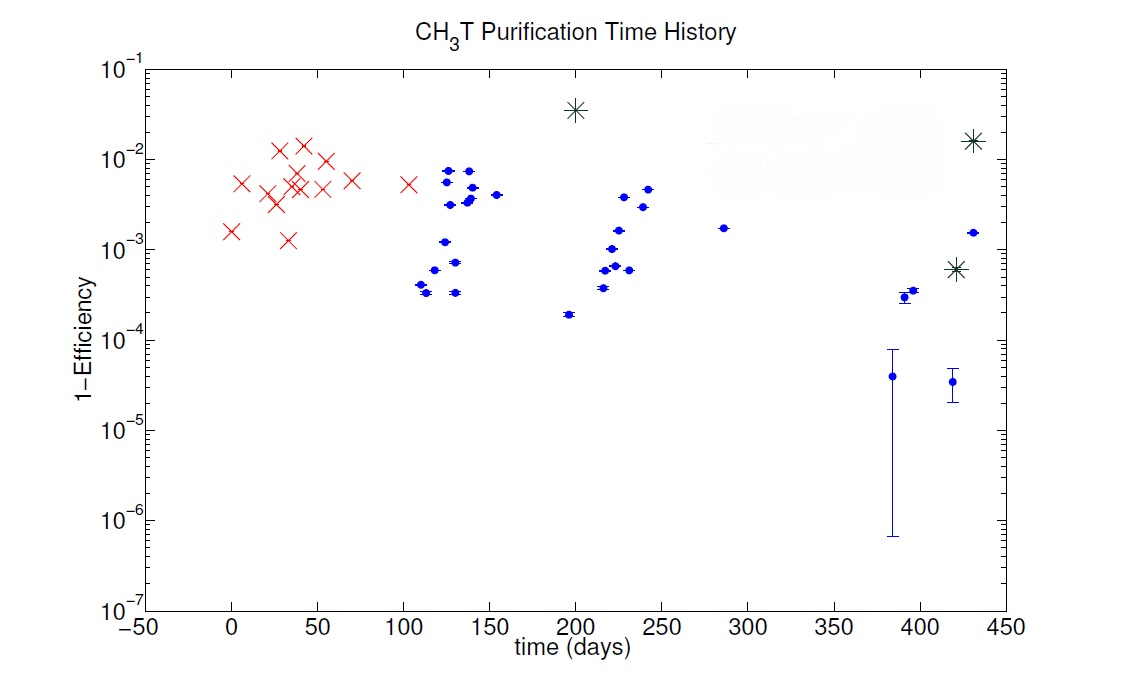
\includegraphics[scale=.45]{GasPhaseRemoval_FlowRate.jpg} 
\captionof{figure}{Single pass inefficiency of the purifier when removing CH$_3$T.  Red and blue points indicate data taken by different students, while the black points indicate data for which procedures were intentionally altered.}
\label{UMDGasFlowRate}
\end{figure}

\begin{figure}
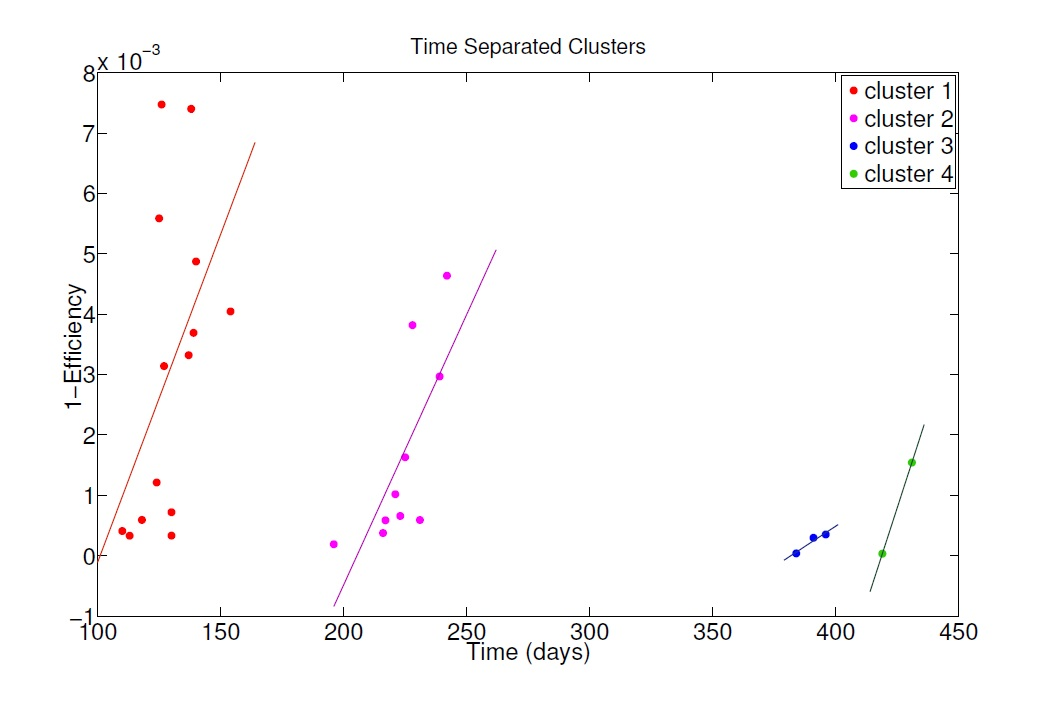
\includegraphics[scale=.4]{GasPhaseRemoval_RestTime.jpg} 
\captionof{figure}{Time-separated clusters of purification have an upward trend in purification inefficiency.}
\label{UMDGasRestTime}
\end{figure}



\subsubsection{Liquid Phase Experiments}

While the gas phase experiments described above showed promising results for the efficient removal of CH$_3$T, they did not account for complexities that appear in LUX, such as the solubility of CH$_3$T in liquid xenon, and the diffusion of CH$_3$T into plastics.  To probe these issues, we also tested tritium removal from a liquid xenon. Our liquid xenon system consists of three main sections: the CH$_3$T injection system, the xenon circulation system, and the liquid xenon cryostat. We will first discuss the set up of the tritium injection system, pictured in Figure~\ref{UMDInjectionSystem}. The injection system begins at the CH$_3$T storage bottle. This bottle is double valved to prevent tritium leakage. As with the gaseous experiments, we have a SAES MC1-905F methane purifier in series with the storage bottle. Following the methane purifier there is a series of injection volumes branching out to the left. These volumes allow us to select how much CH$_3$T to inject into the xenon system. The last component of the injection system is located above the injection volumes. This plumbing is used to collect all of the CH$_3$T from the injection volume via cyropumping. After the plumbing has warmed, the xenon circulating outside of the injection system is rerouted through the cryopump plumbing to sweep all of the CH$_3$T into the xenon circulation system. 


\begin{figure}
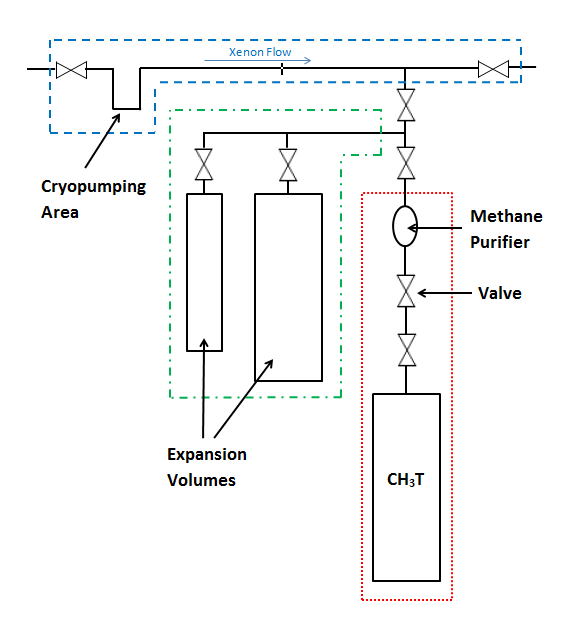
\includegraphics[scale=.6]{UMDInjectionSys.png} 
\captionof{figure}{The tritium injection system for the liquid phase experiments at UMD. The red box indicates the CH$_3$T storage bottle and methane purifier area, the green box indicated the expansion volumes, and the box indicates the cryopumping and xenon flow through area.}
\label{UMDInjectionSystem}
\end{figure}


In the xenon circulation system, a small diaphragm pump circulates gaseous xenon in a closed circuit.  A zirconium getter (SAES PS4-MT3-R-1) is positioned in between the CH$_3$T injection system and the liquid xenon cryostat.  A bypass around the zirconium getter is present to allow control of when CH$_3$T removal occurs.

The final section of our system, the liquid xenon cryostat, is pictured in Figure~\ref{UMDcryo}. In the liquid xenon system, a pulse tube refrigerator cools a xenon gas condenser consisting of a helical coil of copper tubing. The condensed xenon drips into a liquid xenon storage vessel. Two PMTs are placed inside of the storage vessel to observe scintillation light produce by CH$_3$T decays in the liquid xenon. A coincidence is required between the two PMTs to reduce singlet backgrounds in the detector.  Once the vessel is filled both of these PMTs are submerged in the liquid xenon. Note that this means the system at UMD is a single phase detector, rather than a dual phase detector like LUX.  Residual contamination from outgassing plastics was a primary concern for LUX, so 15.75"x2.25"x0.125" polyethylene and teflon curtains were installed in the inner cryostat to surround the PMTs during some of our data sets. These curtains of plastic were used to study outgassing effects in our detector.

\begin{figure}
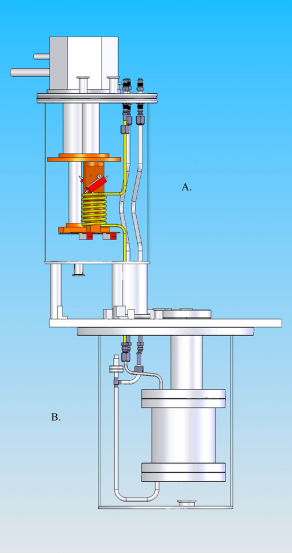
\includegraphics[scale=0.7]{UMDCryo.png} 
\captionof{figure}{The liquid xenon system at UMD. (A) The xenon condenser consists of a helical coil cooled by a pulse tube refrigerator. (B) The liquid xenon storage vessel houses two PMTs to observe tritium decay~\cite{Slutsky:2009gv}.}
\label{UMDcryo}
\end{figure}


During our liquid phase experiments, our experimental procedure consisted of
taking an adequate amount of background data, injecting CH$_3$T into the liquid xenon, waiting for the CH$_3$T event rate to plateau, and then purifying the CH$_3$T
out of the xenon. During the data sets in which teflon or polyethylene curtains
were installed around our PMTs, we bypassed our purifier after initially purifying
away the CH$_3$T so that outgassing effects could be studied. Injection activities for our liquid phase experiment ranged from 1487 $\pm$ 35 Bq to 12164 $\pm$ 1030 Bq.
A detailed list of our purification efficiency measurements in liquid xenon is
shown in Table~\ref{UMDPurification}.  

Using the lessons learned from the gaseous xenon experiments we were able to achieve an average purification efficiency of 99.999\% in our liquid experiments, where we define our purification efficiency to be 

\begin{equation}
\text{Purification Efficiency} = 1 - \frac{A-B}{I-B},
\end{equation}

where A is the background event rate after injecting CH$_3$T, B is the background event rate before to injecting CH$_3$T, and I is the injected CH$_3$T activity as observed by out PMTs. We find that the addition of plastic curtains around our PMTs does not impair our ability to remove CH$_3$T at > 99.998\% levels. To illustrate the effectiveness of CH$_3$T removal, an overlay of injected and purified CH$_3$T spectra is included in Figure~\ref{BeforeAndAfterSpec}. Cumulatively, we have injected over 68,000 observed Hz of CH$_3$T into our liquid xenon. Although systematic errors lead to a fluctuation of our residual background rates, we see no upward trend in our data set as the cumulative observed injection activity rises.(Figure~\ref{UMDBackgroundOverTime})


\begin{figure}
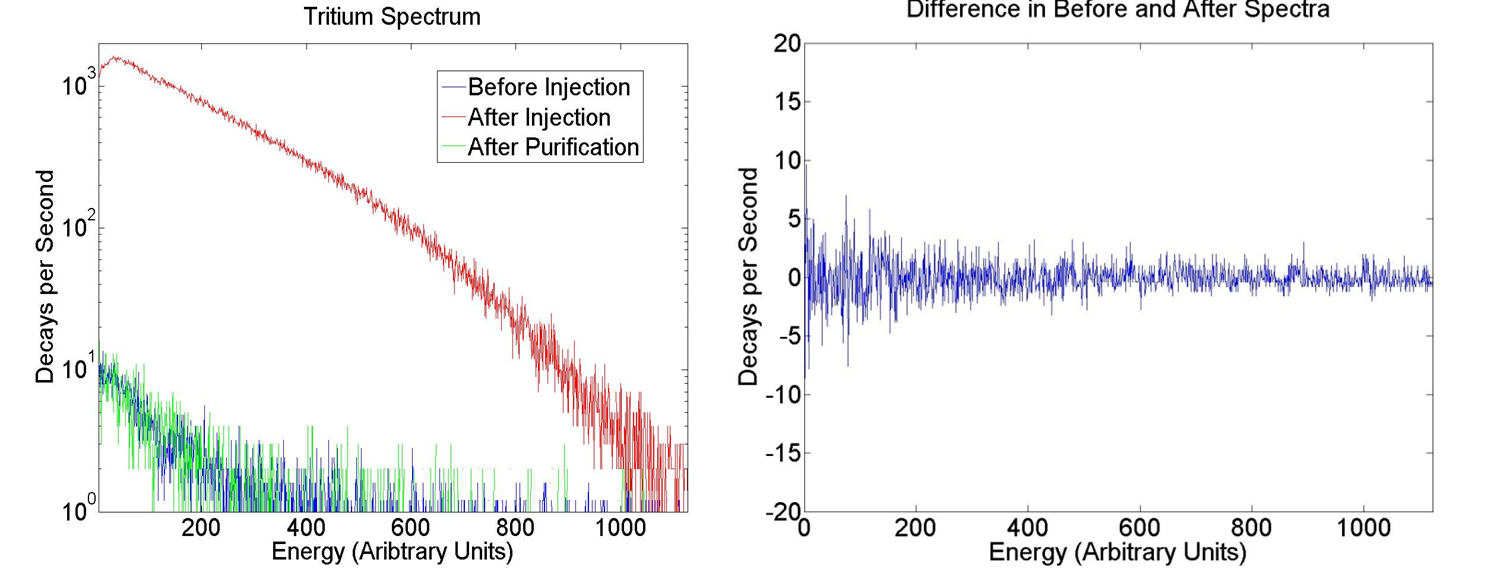
\includegraphics[scale=.5]{UMDspectra.png} 
\captionof{figure}{Left: Overlay of CH$_3$T spectra seen by PMTs in the liquid xenon detector. The blue spectrum is prior to injecting tritium, the red spectrum is after injecting tritium, and the green spectrum is after purifying the xenon. Right: The difference between the before injection and after purification spectra.}
\label{BeforeAndAfterSpec}
\end{figure}

\begin{figure}
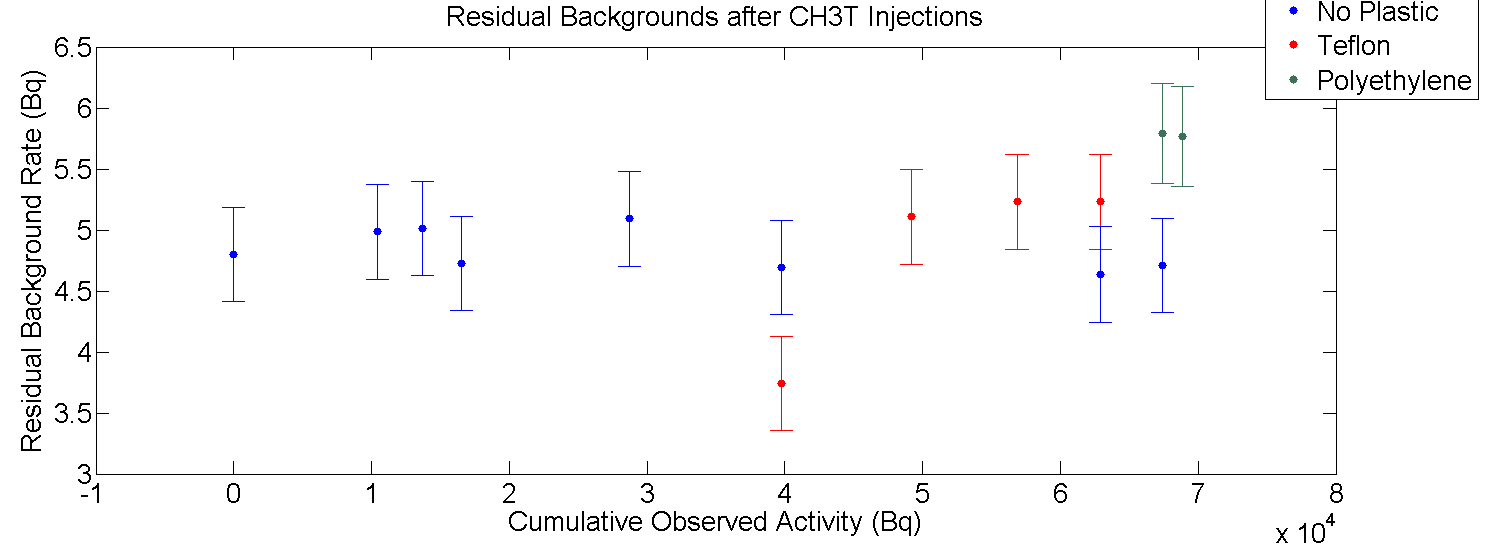
\includegraphics[scale=.35]{ResidualBackgroundCorrected_SystemErr.png} 
\captionof{figure}{Residual background rates over time in the UMD detector after purifying the CH$_3$T out of the xenon. Blue data points are data sets in which no plastic curtains were used inside of the detector, red data points are data sets in which teflon curtains were
used inside of the detector, and green data points are data sets in which polyethylene curtains were used inside of the detector.}
\label{UMDBackgroundOverTime}
\end{figure}

\begin{sidewaystable}
\scalebox{0.8}{
\centering
\caption{CH$_3$T purification efficiencies in liquid xenon. 
Note that the rise in background rate during our polyethylene runs is due to a change in PMT gain. } \label{UMDPurification}
\begin{tabular}{ c | c | c | c | c }
Observed Injection Activity (Bq) & Background Before Injection (Bq) & Background After Injection (Bq) & Purification Efficiency & Type of Plastic \\
\hline
10415.84 $\pm$ 140.89 & 4.78 $\pm$ 0.38 & 4.99 $\pm$ 0.39 & 0.99998 $\pm$ 0.000054 & No Plastic \\
3295.15 $\pm$ 46.28 & 4.99 $\pm$ 0.39 & 5.01 $\pm$ 0.39 & 0.99999 $\pm$ 0.00017 & No Plastic \\
2836.67 $\pm$ 22.35 & 5.01 $\pm$ 0.39 & 4.76 $\pm$ 0.39 & 1.00009 $\pm$ 0.00020 & No Plastic \\
12164.29 $\pm$ 1028.11 & 4.72 $\pm$ 0.39 & 5.09 $\pm$ 0.39 & 0.99997 $\pm$ 0.000082 & No Plastic \\
11033.62 $\pm$ 1766.87 & 5.09 $\pm$ 0.39 & 4.69 $\pm$ 0.38 & 1.00004 $\pm$ 0.00015 & No Plastic \\
9435.13 $\pm$ 180.13 & 3.74 $\pm$ 0.38 & 5.32 $\pm$ 0.39 & 0.99983 $\pm$ 0.000061 & Teflon \\
7666.08 $\pm$ 226.67 & 5.11 $\pm$ 0.39 & 5.23 $\pm$ 0.39 & 0.99998 $\pm$ 0.000082 & Teflon \\
6043.72 $\pm$ 446.80 & 5.23 $\pm$ 0.39 & 5.23 $\pm$ 0.39 & 1.00000 $\pm$ 0.00016 & Teflon \\
4504.81 $\pm$ 220.89 & 4.64 $\pm$ 0.39 & 4.71 $\pm$ 0.40 & 0.99998 $\pm$ 0.00016 & No Plastic \\
1487.09 $\pm$ 35.06 & 5.79 $\pm$ 0.41 & 5.76 $\pm$ 0.41 & 1.00002 $\pm$ 0.00043 & Polyethylene \\
\end{tabular}
}
\end{sidewaystable}


\subsubsection{Outgassing Experiements} 

To more accurately model the LUX detector we surrounded our PMTs with polyethylene or teflon panels during some of our data sets. The experimental procedure for these data sets was to collect an adequate amount of background data, inject CH$_3$T into the liquid xenon, wait for the CH$_3$T event rate to plateau, purify the CH$_3$T away until we reached the initial background event rate, then bypass the purifier on our system to study outgassing effects. Once the purifier had been bypassed we discovered two sources of residual CH$_3$T contamination. We see a gradual rise in CH$_3$T activity after bypassing our purifier due to outgassing of CH$_3$T from the plastic panels.  This outgassing effect will be discussed in detail in Section~\ref{SimOutgas}. In addition to this steady rise, we see large steps in CH$_3$T activity at random intervals. (Figure~\ref{UMDOutgassing}) These step features occur every 3 days on average. The longest period of time without a step occurring was 5.08 days. To examine these step features more closely, we analyzed the spectra from one of these events. We found that the integral of the spectra rose from 8833 $\pm$ 93.98 to 17190 $\pm$ 131.11 during the event, an increase of 194.6\%. (Figure~\ref{UMDOutgassingSpectra})

\begin{figure}
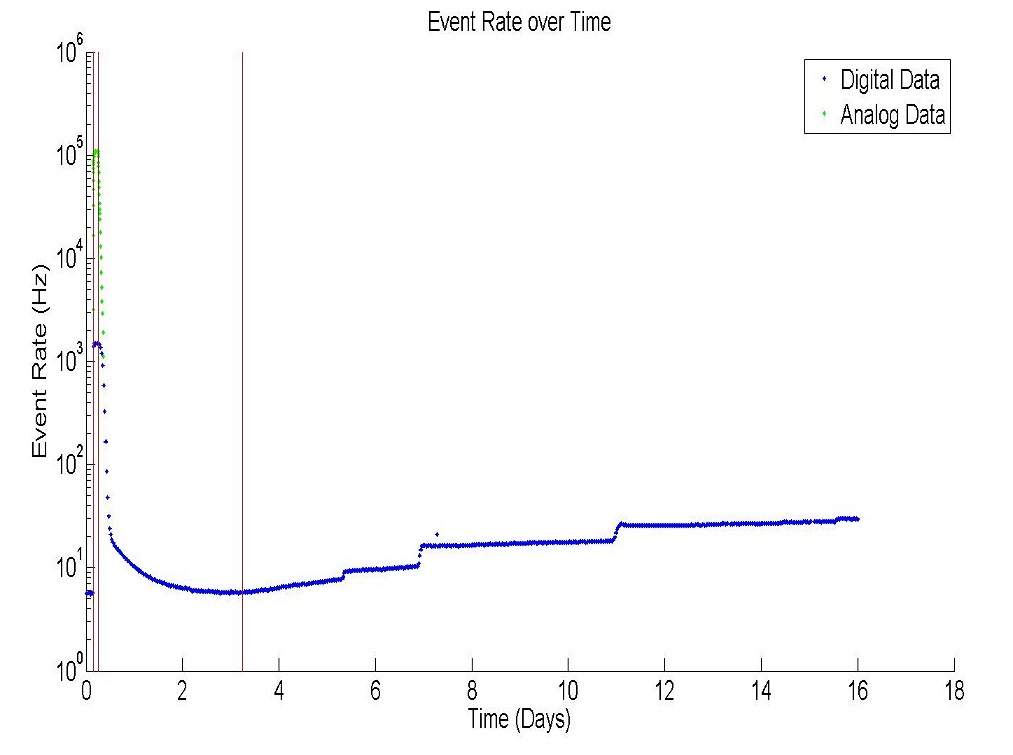
\includegraphics[scale=.35]{Outgassing_TimeHisto_Log.jpg} 
\captionof{figure}{A time histogram of the CH$_3$T rate in our system. The digital event rate was severally limited by dead time in the DAQ, so an analog counter was used to measure the true event rate during the peak of the injection.  The third red line indicates when our purifier was bypassed.  The subsequent rise in the data is due to outgassing of plastics in the detector, while the steps in the data are believed to come from spurts of CH$_3$T entering the cryostat.}
\label{UMDOutgassing}
\end{figure}

\begin{figure}
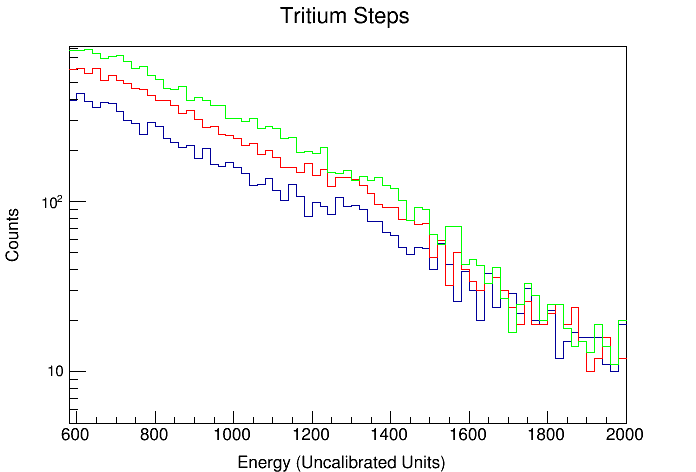
\includegraphics[scale=.35]{Steps_Overlay.png} 
\captionof{figure}{An overlay of three spectra from a step in CH$_3$T after bypassing our purifier. The blue spectrum was collected prior to a step occurring, the red spectrum was collected while a step was occurring, and the green spectrum was collected after the step had reached a plateau.}
\label{UMDOutgassingSpectra}
\end{figure}

Such an increase in CH$_3$T activity can be produced through two mechanisms: a drift in PMT gain which would shift the CH$_3$T spectrum horizontally, or an increase in CH$_3$T activity shifting the CH$_3$T spectrum vertically. To determine if our PMT gain was shifting during our CH$_3$T data sets we used an external $^{137}$Cs source. Over eight days the $^{137}$Cs event rate remained flat, with an initial event rate of 120255 $\pm$ 350 observed Hz and a final event rate of 115469 $\pm$ 339.807 observed Hz. A linear fit to the $^{137}$Cs data results in a nearly zero slope of 0.0026 Hz per day. (Figure~\ref{UMDCsData}) We conclude that the rise in tritium rate during the step events can not be due to our PMT gain drifting, and must therefore be a result of an increase in the amount of CH$_3$T in the fiducial region of our detector. We suspect this increase in CH$_3$T is due to pockets of stagnant gas slowly moving into the detector's fiducial region. To avoid such a source of residual CH$_3$T contamination, a detector wishing to using tritiated methane as an internal calibration source must be designed such that no areas of stagnant gas exist within its system.  

\begin{figure}
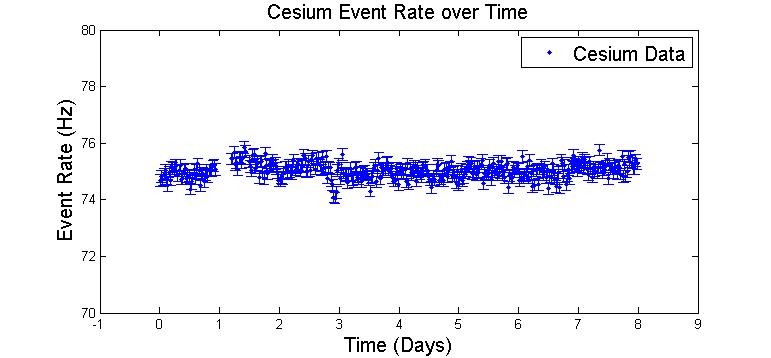
\includegraphics[scale=.35]{Cesium_TimeHisto.jpg} 
\captionof{figure}{The event rate of a $^{137}$Cs source placed outside the xenon storage vessel.  The flatness of the rate over time indicates that the PMT gains are mostly constant.}
\label{UMDCsData}
\end{figure}

\subsubsection{Simulating Outgassing in LUX} \label{SimOutgas}

The outgassing effects seen in UMD's small scale liquid xenon experiment places an upper limit on the CH$_3$T activity that can be injected into low background detectors such as LUX.   In the LUX collaboration we chose to define the tolerable CH$_3$T activity after a calibration to be 5\% of the nominal background rate in LUX, setting a limit on the residual CH$_3$T activity of 0.33 $\mu$Bq.  This upper limit is extremely conservative, and guarantees that any electron recoil backgrounds introduced by a CH$_3$T calibration will be negligible. 

With the above constraints in mind, we can determine an upper limit on the amount of CH$_3$T that can be injected for internal calibrations of the LUX detector. The diffusion process is governed by two different equations known as Fick's laws. Fick's first law describes the flux of a material through a surface. Its general form is given by
\begin{equation}
J=-D\frac{d \phi(r,t)}{d r}.
\end{equation}
Combining Fick's first law with the continuity equation given by
\begin{equation}
\frac{\delta \phi}{\delta t} + \nabla \cdot J = 0,
\end{equation}
which states that a change in density in any part of the system is due to inflow and outflow of material results in Fick's second law,
\begin{equation}
\frac{\delta \phi}{\delta t} = D \nabla^2 \phi,
\end{equation}
which describes the transport of a material by diffusion.

To implement these diffusion laws into our model we must determine the diffusion coefficient of CH$_3$T in the plastics of LUX. At room temperature, the diffusion coefficient of methane in teflon is measured to be $2.3 \times 10^{-7}$ cm$^2$/sec~\cite{MethaneDiffusion}.  The temperature dependence of this diffusion constant is modeled by the Arrhenius equation,  
\begin{equation}
D=Ae^{\frac{-E_a}{RT}}
\end{equation}
where $E_a$ is the activation energy, $R$ is the gas constant, and $T$ is the temperature.  Assuming an activation energy of 41.3 kJ/mol (from~\cite{TeflonActivationEnergy}), this suggests that an adjustment factor to the diffusion constant of $10^6$ at liquid xenon
temperature. This adjustment factor is equivalent to increasing the thickness of the plastic in our model by a factor of 1,000. For this reason we are motivated
to use half-infinite line boundary conditions in our diffusion model.

The analytic solution to Fick's second law using half-finite line boundary conditions is
\begin{equation}
\phi(x,t) = KC_{out} - \int_0^t \text{erf}\left(\frac{x}{\sqrt{4D(t-\tau))}}\right)K \dot{C_{out}}(\tau)d\tau - KC_{out}(0)\text{erf}\left(\frac{x}{\sqrt{4Dt}}\right)
\end{equation}
where $K$ is the solubility of the material and $C_{out}$ is the outside concentration of the material.  For the outgassing process we are only interest in the flux of the material out of the plastic.  This is given by Fick's first law evaluated at $x=0$,
\begin{equation}
J_{out}(t)=-K\sqrt{\frac{D}{\pi}} \left( \int_0^t \frac{\dot{C_{out}(\tau)}}{\sqrt{t-\tau}}d\tau + \frac{C_{out}(t)}{\sqrt{t}} \right),
\end{equation}
where the sign has been flipped since the flux of material is outward. We see that it is not possible to measure $K$ and $D$ separately. To simplify our notation, we define a new constant
\begin{equation}
G=K\sqrt{\frac{D}{\pi}}.
\end{equation}
We can fit the integral of our equation for the flux out of the plastic over time to the outgassing data collected in the liquid xenon system to extract a value for the constant $G$. Since the outgassing data includes step features from stagnant pockets of unpurified CH$_3$T, we can set an upper limit on $G$ by assuming the step features are a result of outgassing itself, and a lower limit on $G$ by removing the steps from our data, treating them as if they have no connection to outgassing at all. With this method
we loosely constrain $0.0001 \frac{\text{cm}}{\sqrt{\text{day}}} \le G \le 0.0075  \frac{\text{cm}}{\sqrt{\text{day}}}$ (Figure~\ref{StepsandNoSteps}). The value of G was further constrained to $G \le 0.0002 \frac{\text{cm}}{\sqrt{\text{day}}}$ by injecting natural methane into LUX and observing the effects of outgassing with the sampling system. 

\begin{figure}
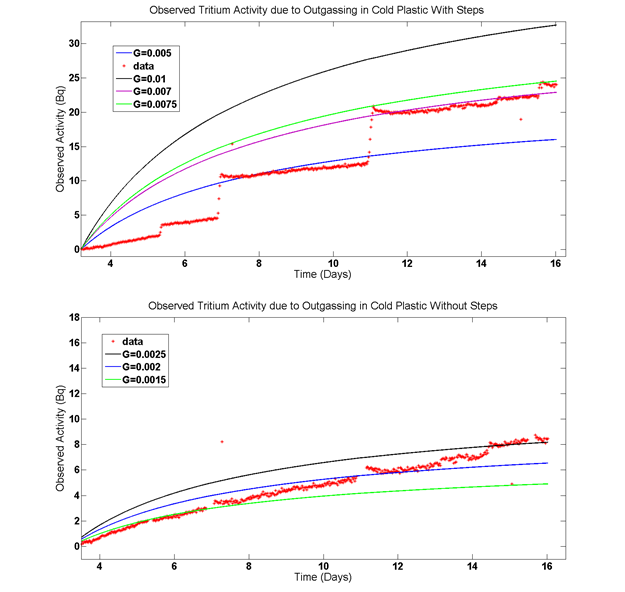
\includegraphics[scale=.7]{StepsandNoSteps.png} 
\captionof{figure}{Fits of the integral of the flux of CH$_3$T out of plastic over time to the outgassing data collected in Maryland's liquid xenon system assuming that the step features
are due to diffusion. The model does not perfectly describe the data, so a range of $G$ values is shown. These fits are used to
set an upper limit on $G$. Bottom: Fits of the integral of the flux of CH$_3$T out of plastic over time to the same data, assuming that the step features are not due to diffusion. These fits are used to set a lower limit on $G$.}
\label{StepsandNoSteps}
\end{figure}


With a constraint on G taken from the analytic solution to Fick's second law, we turn to numerical simulation to answer
the question of how much initial CH$_3$T activity can be injected into LUX without violating our background rule. Several assumptions are made to simplify the numerical model. First, we approximate the diffusion into plastic as being a one dimensional process. In cylindrical coordinates, Fick's laws become
\begin{equation}
J = -D \left( \frac{\delta \phi}{\delta r} \mathbf{\hat{r}} + \frac{1}{r} \frac{\delta \phi}{\delta \theta} \boldsymbol{\hat{\theta}} + \frac{\delta \phi}{\delta z} \mathbf{\hat{z}} \right) 
\end{equation}
\begin{equation}
\frac{\delta \phi}{\delta t} = D \left( \frac{\delta^2 \phi}{\delta r^2} + \frac{1}{r}\frac{\delta \phi}{\delta r} + \frac{1}{r^2} \frac{\delta^2 \phi}{\delta \theta^2} + \frac{\delta^2 \phi}{\delta z^2} \right).
\end{equation}
Since the plastic in our detector at Maryland and in LUX can be approximated by a cylindrical shell, there is no dependence on the azimuthal or z coordinates. Since $r$ is large compared to the thickness of the plastic shell, $\frac{\delta^2 \phi}{\delta r^2} \gg \frac{1}{r}\frac{\delta \phi}{\delta r}$, so we can make the approximations
\begin{equation}
J=-D\frac{\delta \phi}{\delta r} \mathbf{\hat{r}}
\end{equation}
\begin{equation}
\frac{\delta \phi}{\delta t} = D \frac{\delta^2 \phi}{\delta r^2}
\end{equation}

We assume the concentration of CH$_3$T in LUX is uniform throughout its volume. This assumption is justified, since the design of LUX creates currents which stirs the liquid xenon. With perfect mixing the effect of the purifier can be modeled by adding an exponential time dependence to the concentration in the liquid xenon.  We expect the time constant of this decay is equal to the time it takes xenon to recirculate through the LUX detector. We use a simple implementation of the first order Euler method for our numerical simulations. The finite difference approximations of Fick's two laws in one dimension are
\begin{equation}
J_{i,j}=-D \frac{ \phi_{i+1,j} - \phi{i,j}}{\Delta x}
\end{equation}
\begin{equation}
\phi_{i,j+1}=\phi_{i,j}+ \Delta t \left( \frac{\phi_{i+1,j}-2\phi_{i,j}+\phi_{i-1,j}}{\Delta x^2}\right)
\end{equation}
where $i$ is the spacial index and $j$ is the time index.  To avoid divergent solutions we need
\begin{equation}
D\frac{\Delta t}{\Delta x^2} \le \frac{1}{2}.
\end{equation}
For effects to be propagated across N spatial bins, N time steps are required.
Therefore, the effective time resolution is
\begin{equation}
\Delta t_{\text{effective}}=\Delta t \times N_x.
\end{equation}

The diffusion is simulated by setting the concentration at the boundary of the piece equal to $KC_{out}$, where $C_{out}$ is the concentration of CH$_3$T in the liquid xenon. This concentration is dependent on time according to
\begin{equation}
\frac{\delta C_{out}}{\delta t} = J_{out} \frac{A_{\text{plastic}}}{V_{\text{xenon}}}-\frac{C_{out}}{\tau}
\end{equation}
where $A_{\text{plastic}}$ is the surface area of the LUX plastic, $V_{\text{xenon}}$ is the total volume of xenon in the fiducial region, and $\tau$ is the time it takes for one full purification cycle. 

It was originally assumed that $\tau$ would equal the turn over time of the xenon circulation system in LUX ($\sim$ 1.3 days), but was later found that $\tau$ was much shorter than expected ($\sim$ 6 hours).  While the exact reason for this is not understood, it is likely due to the complex circulation path of the LUX xenon through the PMT purge lines, or due to an over abundance of CH$_3$T in the gas phase.

The first term on the right of this equation models outgassing of CH$_3$T from the plastic cylinder, while the second term models removal of CH$_3$T through purification. Using the first order Euler method, we arrive at an expression for $C_{out}$ given by
\begin{equation}
C_{j+1}=C_j + \Delta t \left[\left( J_{1,j}-J_{N_x,j}\right) \frac{A_{\text{plastic}}}{V_{\text{xenon}}} - \frac{C_j}{\tau} \right].
\end{equation}

The initial concentration is defined by dividing the desired injection activity by the volume of the fiducial region. We choose $D = 2.3 \times 10^{-9} \frac{\text{cm}^2}{\text{sec}}$ such that the
half-infinite boundary conditions in our diffusion model is valid, and combine this with our allowed range of values for $G$ to extract a value for $K$. We find that an initial injection activity of 10 Bq results in the background rate returning to $<$ 5\% of its initial value in one month~\cite{JonOutgassing}. (Figure~\ref{OutgassingSim})

\begin{figure}
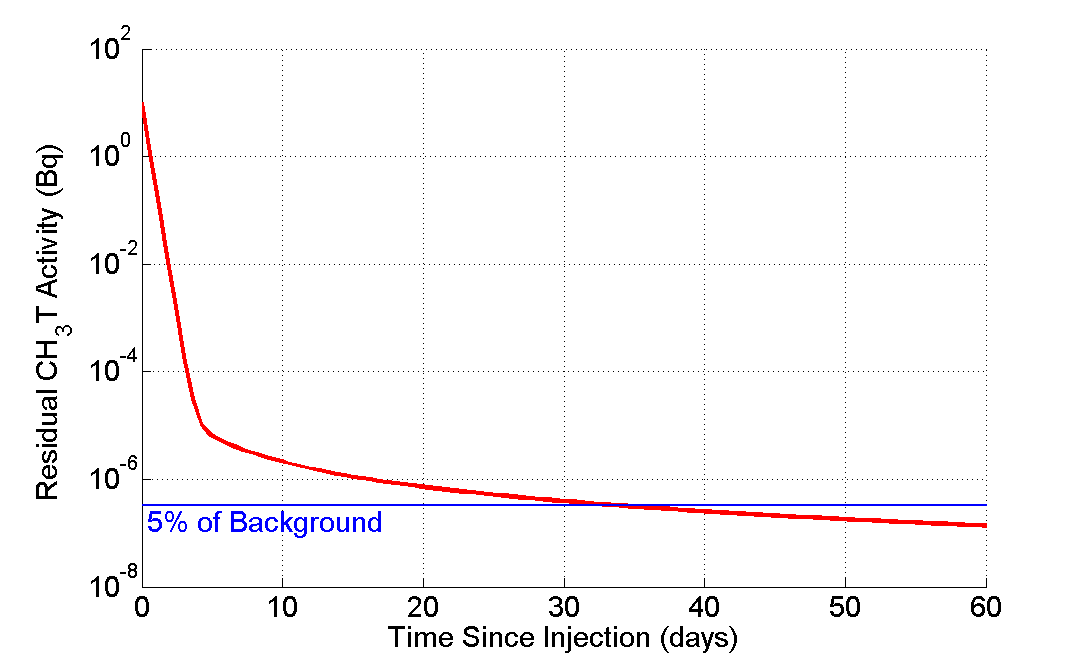
\includegraphics[scale=.3]{OutgassingSim.png} 
\captionof{figure}{The results of simulating the CH$_3$T activity in LUX after a 10 Bq injection.  In the first week the amount of residual CH$_3$T is dominated by the purification time constant, while the outgassing time constant determines the amount of activity later times.}
\label{OutgassingSim}
\end{figure}


\subsection{Injection of Tritiated methane into LUX}

The hardware of our tritiated methane calibration technique can be separated into three parts: the injection system, the tritiated methane source bottle, the zirconium getter.

The tritiated methane source bottle was prepared in three steps. First, we prepared a xenon bottle that had similar pressure and purity to the LUX system. We filled a 2250 cc stainless steel bottle with 1590 torr of xenon from the same dekryptonation and purity program from which the LUX xenon came. This xenon was to serve as a carrier gas for the tritiated methane. 

The next step was to prepare a small amount of tritiated methane to mix with this dekryptonated xenon. A reservoir of tritiated methane with an activity of 204 Bq/torr-cc was purchased from Moravek Biochemical. The reservoir was frozen with liquid nitrogen, resulting in a vapor pressure of 10.4 $\pm$ 0.05 torr.  We then opened the frozen tritiated methane reservoir to a number of expansion volumes so that a small amount of activity could be extracted.  The first expansion volume was a 1/4" VCR cross which was sealed with swagelok valves on each side, and had a total volume of 5.2 $\pm$ 0.9 cc. Next, we isolated the VCR cross from the tritiated
methane reservoir and then opened it to a 501 $\pm$ 0.2 cc expansion volume. We isolated the VCR cross a second time and then opened it up to a 53.2 $\pm$ 3.4 cc expansion volume. The VCR cross was then isolated for a third time before opening it to a 10.5 $\pm$ 0.5 cc expansion volume. After this final expansion the VCR cross was isolated and the remaining 0.016 $\pm$ 0.006 torr-cc of tritiated methane left within was mixed with the dekryptonated xenon inside the 2250 cc bottle via cryopumping. The final result was a tritiated methane source which had an activity of 9.1e-7 $\pm$ 3.4e-7 Bq/torr-cc ($\sim$3.3 torr total).  After the success of the initial CH$_3$T calibrations in LUX, a similar procedure was used to produce a 300 Bq source bottle for higher statistics calibrations.

The injection system for our tritiated methane calibration technique consists of a series of expansion volumes which are used to fine tune the amount of CH$_3$T that is injected (Figure~\ref{LUXInjectionSys}). Once the CH$_3$T source bottle is opened the xenon gas and CH$_3$T flows through a methane purifier (SAES MC1-905F) to remove any sources of potential contamination, such as bare tritium. The CH$_3$T then flows into the expansions volumes set by the
user. We use expansion volumes of 9.8 $\pm$ 0.4 cc, 13.3 $\pm$ 0.4 cc, 26.0 $\pm$ 0.5 cc, 82.7 $\pm$ 0.5 cc, 12.0 $\pm$ 0.6 cc, and 132.7 $\pm$ 0.6 cc, which provide over an order of magnitude control in the strength of an injection. Note that each injection will lower the remaining activity in the CH$_3$T source bottle via volume sharing, resulting in a smaller, yet calculable, injection activity with subsequent injections. Once the expansion volumes
have filled, the flow of xenon in the gas system is diverted through the expansion volumes to sweep the CH$_3$T into the detector. We continue to flow through the expansion volumes for one hour at 1 SLPM, which is equivalent to flushing out the full 384.5 cc of the expansion volumes roughly 75 times. Two pump out ports allow various parts of the injection system to be evacuated in preparation for each use. A pressure gauge (PT-T1) is included above the tritiated methane source
bottle so that this drop in activity can be measured. The final component of the injection system is a particle filter (Mott Corp. GSP3752FF11) which prevents particles contaminants from entering the LUX detector.

\begin{figure} [!h]
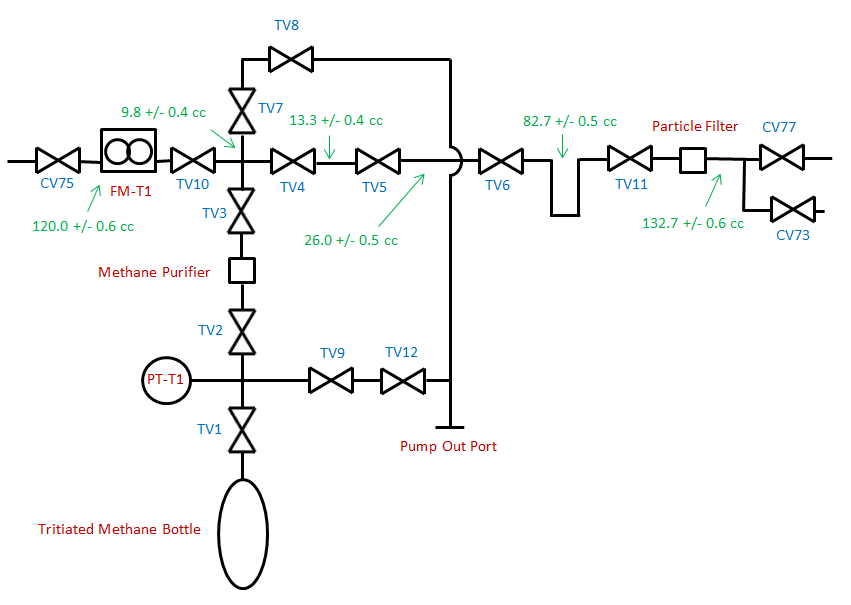
\includegraphics[scale=.6]{TritiumPlumbing.png} 
\captionof{figure}{Plumbing diagram of the LUX tritium injection system.  Blue labels indicate valves, red labels indicate equipment, and green labels indicate the size of individual expansion volumes when all valves are closed.}
\label{LUXInjectionSys}
\end{figure}

Once the CH$_3$T has been injected in the LUX gas system it flows into the liquid xenon inside of the LUX cryostat, where it mixes uniformly throughout the fiducial volume.  Since the xenon gas in LUX is constantly circulating, the remaining CH$_3$T is swept out of inner cryostat with the circulating xenon.  The LUX gas system uses a hot zirconium getter (SAES PS4-MT15-R-1) downstream of the cryostat to remove CH$_3$T and other impurities from from the xenon. Extensive R\&D was conducted using a smaller zirconium getter (SAES PS4-MT3-R-1) at the University of Maryland to learn about the CH$_3$T removal efficiency of these purifiers. Details of these studies is discussed in section~\ref{UMDRemoval}.


\subsection{ER Band Calibration of the LUX Detector} \label{DiscrimSec}

The LUX collaboration took many precautions to ensure a safe and successful tritium injection. Prior to injecting any tritiated methane into the detector, a natural methane injection was performed to measure the purification time constant in LUX and constrain the value of $G$ further.   Twenty milligrams of natural methane were injected into LUX using the CH$_3$T injection system. The sampling system was used to measure the concentration of methane in the detector over the next few days, and a purification time constant of 5.90 $\pm$ 0.07 hours was measured.  The first natural methane injection was not large enough to observe outgassing from the detector, but a larger natural methane injection of 0.375 grams was able to constrain $G \le 0.0002 \frac{\text{cm}}{\sqrt{\text{day}}}$ at a later date.


\begin{figure} [!h]
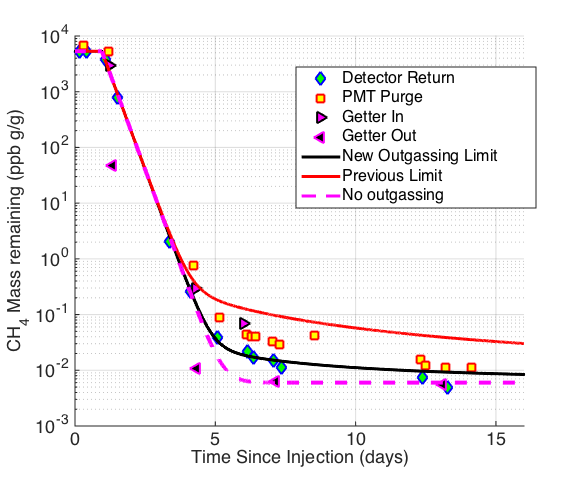
\includegraphics[scale=.7]{LUXOutgassing.png} 
\captionof{figure}{Sampling system results from the 0.375 gram natural methane injection performed in April 2015.  The various symbols represent different sampling locations throughout the detector.  The results were used to constraint the value of $G$~\cite{JonOutgassingTwo}.}
\label{LuxOutgassing}
\end{figure}

After the natural methane campaign a small amount of tritium was injected into LUX to confirm the purification time constant from above, and to confirm the mixing of the source throughout the detector.  A fiducial volume containing 125 kg of xenon between drift times of 30 to 320 $\mu$sec, with radius $ < $17.5 cm was defined for the analysis.  The first 23 hours of data show that the initial injection activity in the fiducial volume was 24.2 $\pm$ 0.3 mHz, while the initial injection activity in the entire detector was 44.9 $\pm$ 0.5 mHz.  The ratio of the fiducial volume activity to the total volume activity is 0.539 $\pm$ 0.009, which is close to the expected ratio of 0.5 for a perfectly uniform distribution of CH$_3$T events. The CH$_3$T activity fell with a purification time constant of 6.9 $\pm$ 0.4 hours within the fiducial volume, confirming the $\sim$ 6 hour time constant measurement.

\begin{figure} [!h]
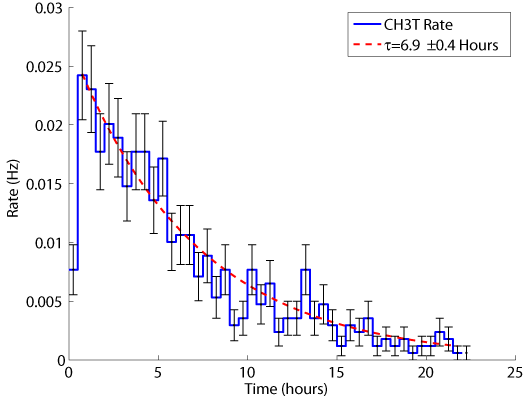
\includegraphics[scale=.7]{CH3T_fid_rate_new.png} 
\captionof{figure}{Rate of CH$_3$T events after the first small injection into LUX.  The 6.9 hour time constant is consistent with expectations from the natural methane sampling campaign prior to this injection.}
\label{LUXPurificationRate}
\end{figure}

After confirming the purification time constant, the LUX committee approved the use of CH$_3$T as an internal calibration source.  The initial CH$_3$T calibration was limited to 0.3 Hz due to the uncertainty in the value of the the diffusion constant $G$, but injections ranging from 2-10 Hz have been done every 3-4 months after the value of $G$ was constrained further.  The location of events from the first CH$_3$T calibration is shown in Figure~\ref{TritiumSpatialDist}. As expected, the CH$_3$T source mixes uniformly throughout the detector.  
\begin{figure} [!h]
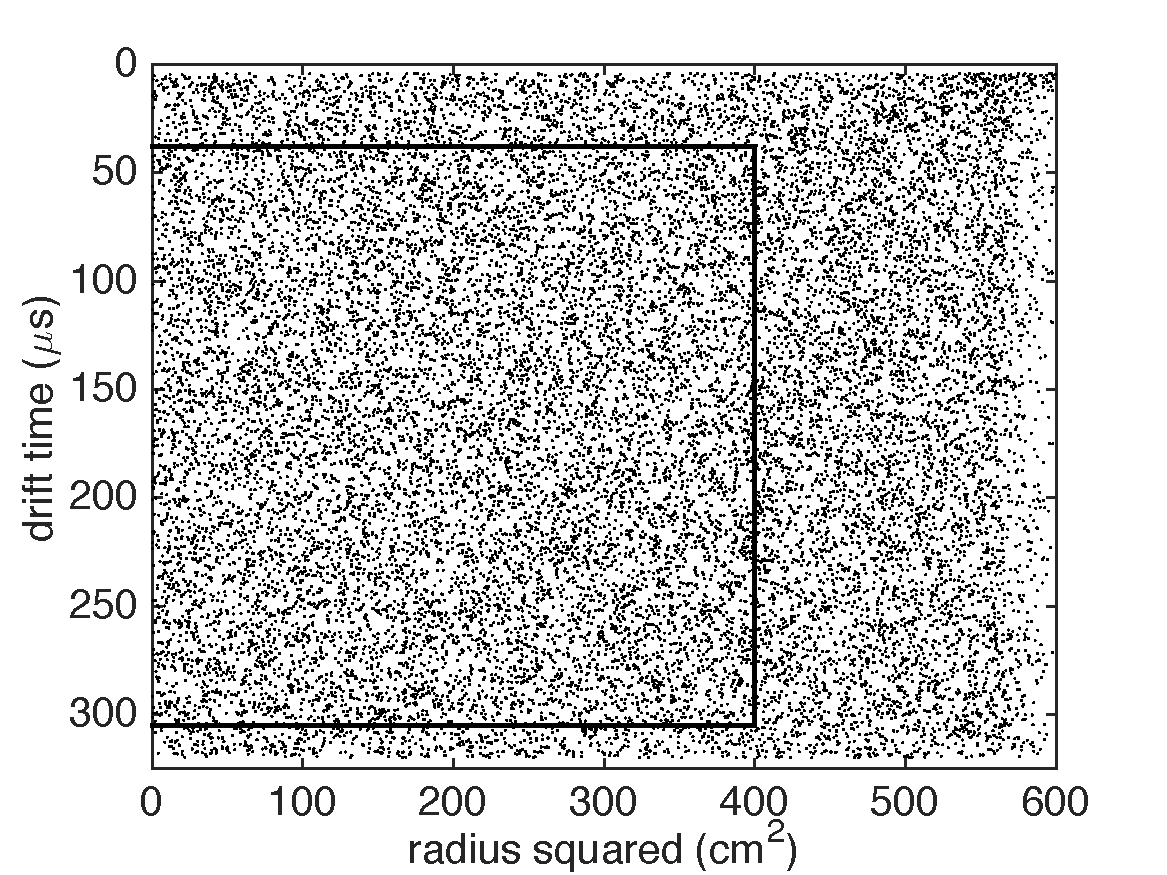
\includegraphics[scale=.5]{TritiumRvZ.pdf} 
\captionof{figure}{The location of events during the August 2013 LUX CH$_3$T injection.  The solid black like indicates the fiducial volume used for the first LUX Run3 results paper.}
\label{TritiumSpatialDist}
\end{figure}

The combined energy spectrum for a high statistics CH$_3$T calibration is shown in Figure~\ref{TritiumSpectrum}.  A model of the expected tritium beta spectrum which includes detector resolution effects is shown in red.  The data agrees very well with expectations above the detector's energy threshold, with a p-value of 0.70 from 3 to 18 keV.  The consistency of the energy spectrum across a wide range of energies provides strong support for the combined energy model presented in Section~\ref{CombinedEnergyModel}.  The ratio of the CH$_3$T data to expectations was used to determine the energy threshold of the LUX detector.  An error function fit determines a 50\% energy threshold of 1.24 $\pm$ 0.026 keV for electron recoil events.


\begin{figure} [!h]
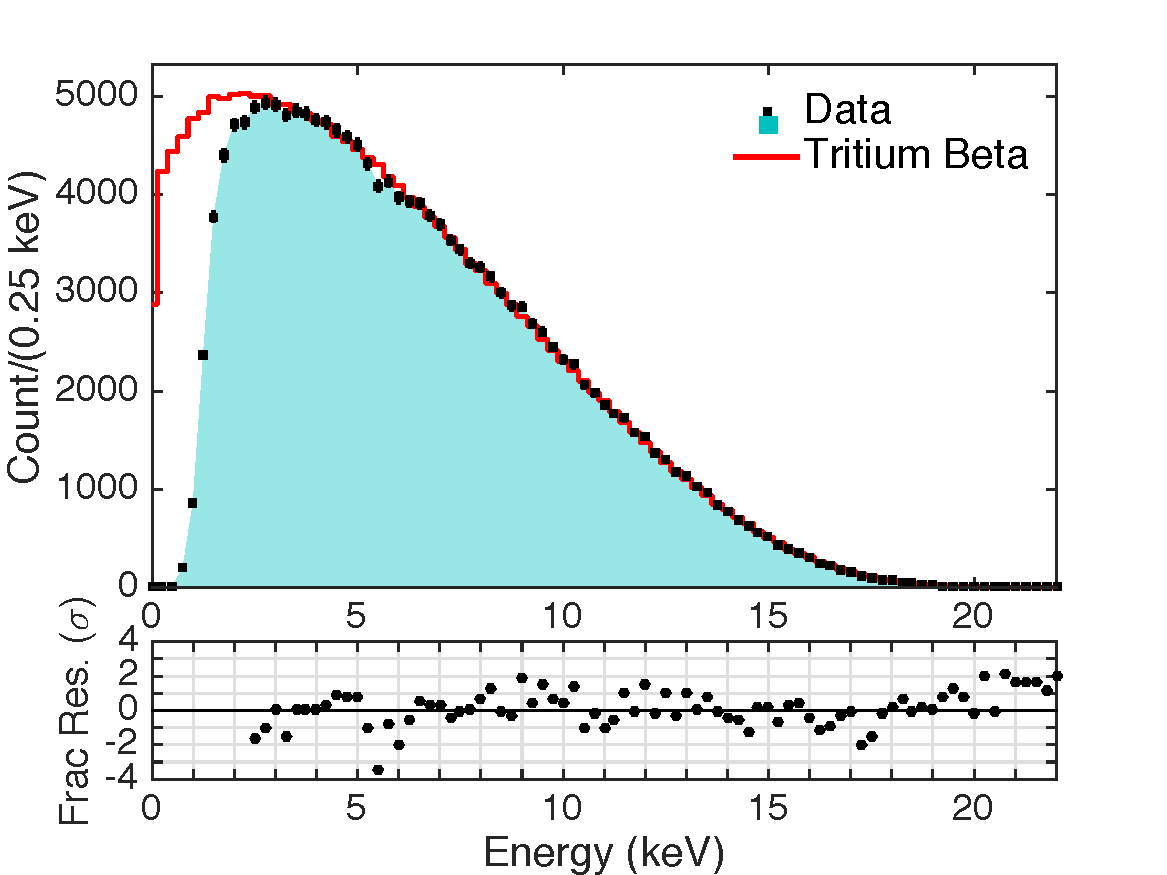
\includegraphics[scale=.425]{TritiumSpectrum.pdf} 
\captionof{figure}{Top: The combined energy spectrum from a high statistics CH$_3$T calibration in LUX taken in December 2013.  Data is shown in black, and a model of the expected tritium beta spectrum is shown in red.  Bottom: The residual differences between the data and model for each bin, in units of $\sigma$.}
\label{TritiumSpectrum}
\end{figure}

\begin{figure} [!h]
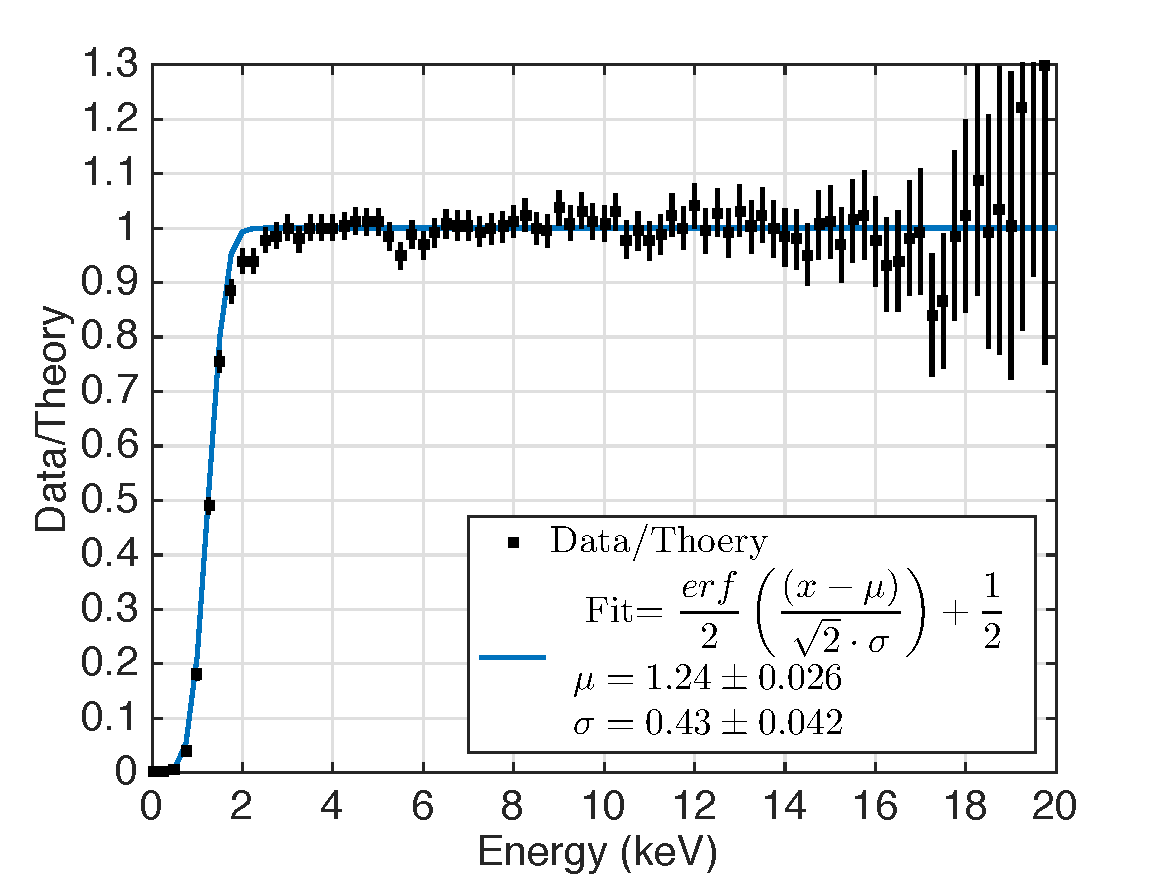
\includegraphics[scale=.4]{TritiumThreshold.pdf} 
\captionof{figure}{The ratio of the tritium data to expectations.  An error function fit used to determine the energy threshold is shown in blue.}
\label{TritiumThreshold}
\end{figure}

The main purpose of the CH$_3$T calibration source is to measure the detector's electron recoil response.  This calibration is crucial when determining the "leakage fraction" of electron recoil backgrounds that fall below the nuclear recoil band mean.  Alternatively, a "discrimination" factor can be defined as the fraction of electron recoil backgrounds that do not fall below the nuclear recoil band mean.  The electron recoil band from a high statistics CH$_3$T calibration is shown in Figure~\ref{TritiumERBand}.  The nuclear recoil band calibration from LUX's neutron generator calibration source is also included in Figure~\ref{TritiumERBand}. These two results have allowed the LUX collaboration to measure the detector's discrimination with unprecedented accuracy.  An average discrimination (1-$f$) for the LUX Run3 result was found to be 99.81\% $\pm$ 0.02\%.

In addition to the calibration results mentioned in this section, the CH$_3$T calibration source has allowed the LUX collaboration to measure fundamental properties of liquid xenon to high accuracy.  These results are discussed in reference~\cite{TritiumPaper}.  The calibration source is also an integral part of producing signal corrections in a detector with a nonuniform electric field, a topic which is discussed in chapter~\ref{Run04Corrections}.


\begin{figure} [!h]
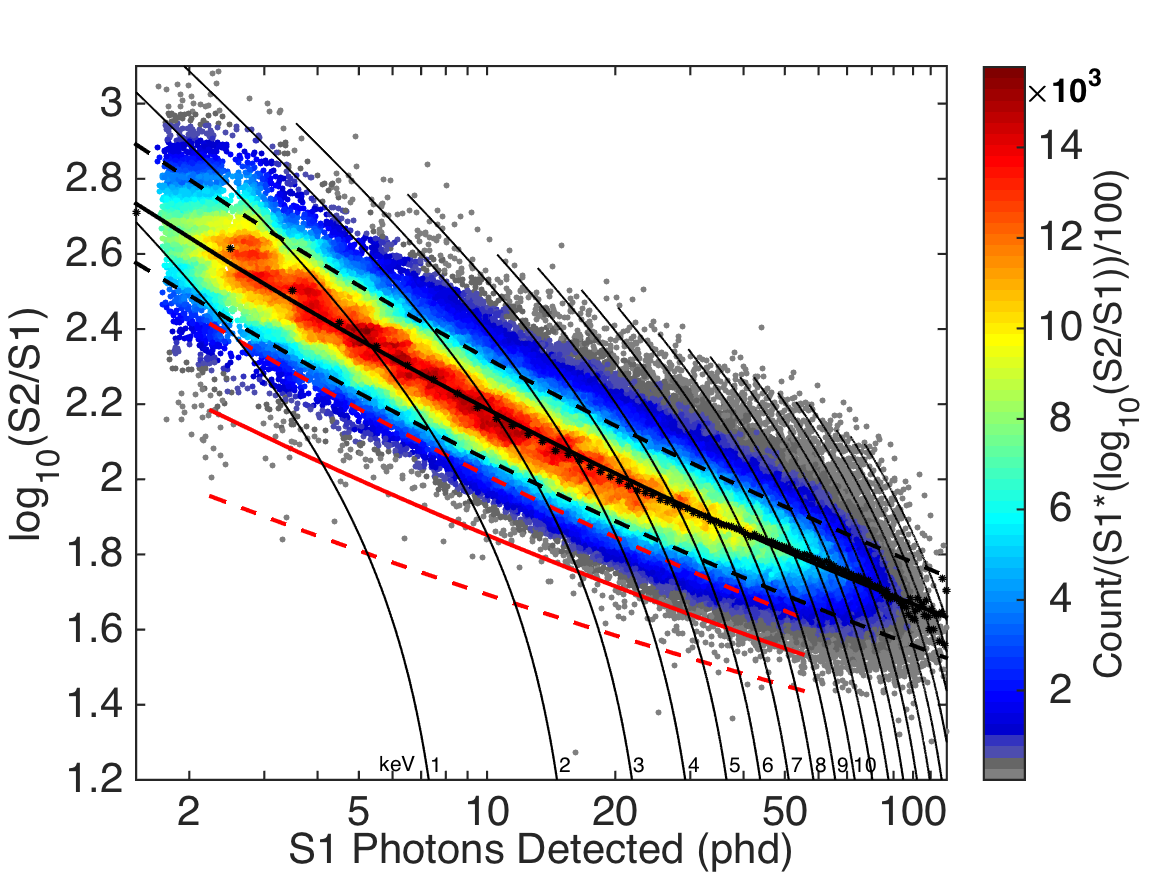
\includegraphics[scale=.35]{TritiumERBand.pdf} 
\captionof{figure}{The electron recoil calibration of LUX resulting from 170,000 CH$_3$T events at 180 V/cm.  The Gaussian means of each S1 bin, as well as power law fits to those means and the 10\% and 90\% contours of the ER band are shown in black.  The power law fits to the mean, 10\%, and 90\% contours of the NR band are shown in red.}
\label{TritiumERBand}
\end{figure}

\begin{figure} [!h]
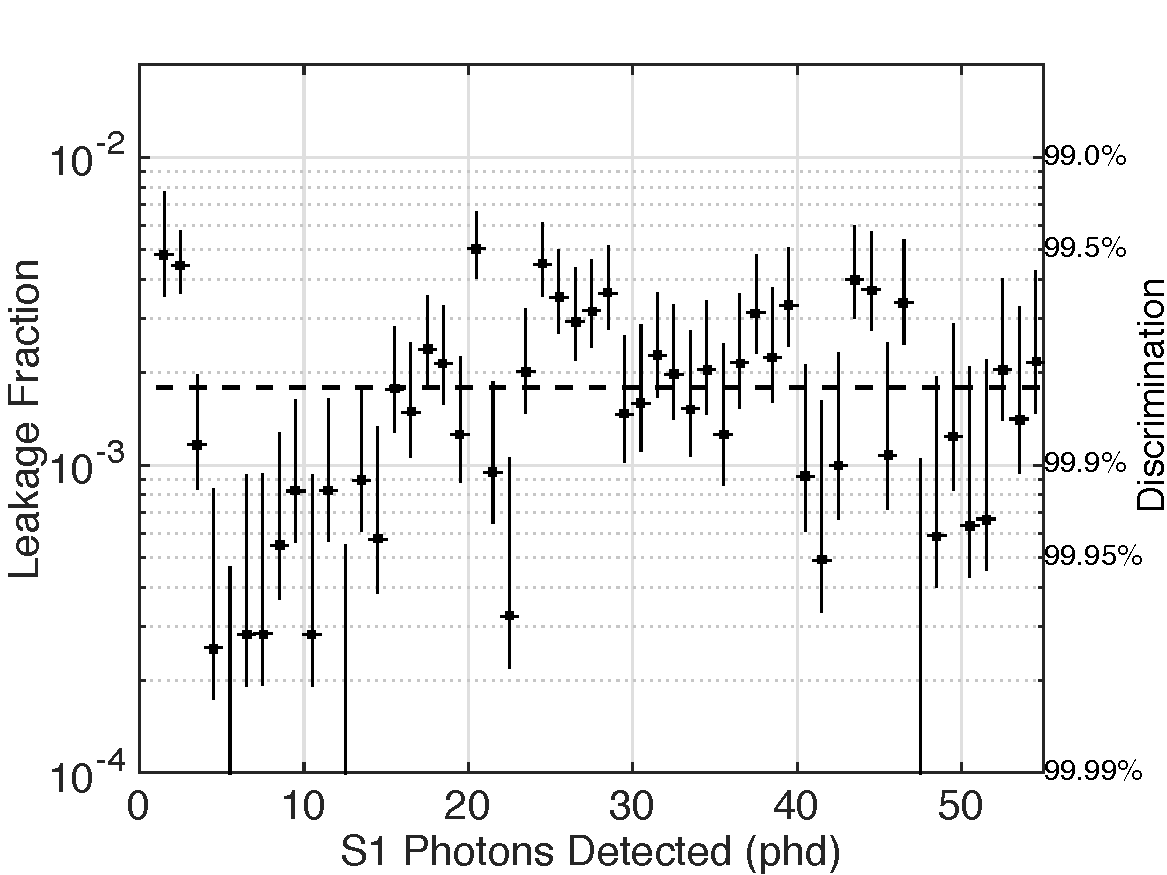
\includegraphics[scale=.35]{TritiumLeakage.pdf} 
\captionof{figure}{The leakage fraction and discrimination versus S1 in the LUX detector at 180 V/cm.}
\label{TritiumLeakage}
\end{figure}